% TeXiFy 似乎无法正确解析 *.tex 和 thesis-ref.bib 的关联,导致误报 UnresolvedReference
%! suppress = UnresolvedReference


\chapter{绪论}\label{ch:intro}


\section{\app 的背景与意义}\label{sec:background}

\subsection{国内外心血管疾病现状}\label{subsec:disease}

根据中国国家心血管病中心出版的《中国心血管健康与疾病报告2021》\cite{Zhongguoxinxieguanjiankangyujibingbaogao20212022},目前中国人口心血管疾病的发病率和患病率均处于持续上升阶段,心血管疾病已成为居民死亡的首位原因;2019年,中国农村、城市心血管疾病分别占死因的46.74\%和44.26\%。心血管疾病给社会和居民带来的经济负担日益加重,且杀伤力越来越强。

不仅如此,根据世界卫生组织的统计,心血管疾病也是全球的头号死因,每年死于心血管疾病的人数多于任何其它死因;2019年,估计有1790万人死于心血管疾病,占全球死亡总数的32\%\cite{CardiovascularDiseasesCVDs}。

同时,近年来新型冠状病毒(COVID-19)的爆发也加剧了心血管疾病的危害。证据显示,既往合并心血管疾病的患者更容易在新型冠状病毒感染后发展为重症患者,死亡风险更高,体征和症状更容易恶化\cite{zhangXinxingguanzhuangbingdufeiyanyuxinxieguanjibing2020}。

\subsection{心电监测的用途与原理}\label{subsec:monitoring}

尽早发现心血管疾病非常重要,这样就可以及时采取措施,减少疾病对患者健康的威胁\cite{CardiovascularDiseasesCVDs}。在各种心血管疾病的诊断方法中,心电图(Electrocardiogram,缩写为ECG)是最常用、最基本、最重要的一种,具有非侵入性、诊断快速、成本低廉、广泛可用等诸多优点\cite{Xinxieguanjibingzhenduanliuchengyuzhiliaocelue2007}。

心电图是对心电信号的记录。通过放置在皮肤上的电极可以检测到心脏的电活动,将电压与时间的关系绘制为二维图像就得到了心电图。

\subsection{常规心电图与动态心电图}\label{subsec:standard-holter}

心电图有两种主要类型:常规心电图(Standard ECG)和动态心电图(Holter ECG、Dynamic ECG或Ambulatory ECG)。

常规心电图,也被称为静息心电图(Resting ECG),是在患者保持静止状态时记录的心电图。常规心电图的记录需要在专业的医疗机构中进行,患者通常处于平躺状态,在四肢和胸部表面安装电极,电极检测心脏产生的电信号并将其传输到心电图仪器。常规心电图通常包含12个导联\footnote{这里的一个导联是指一对电极之间的电势差,比如Ⅱ导联是指右臂电极和腿电极之间的电势差。另外,连接电极与心电图仪器的电缆也常被称为导联。本文中无特别说明的情况下,导联均指电势差而非电缆。},一次记录10秒,并打印在心电图纸上,如图~\ref{fig:ecg-paper-example} 所示是一张10秒12导联的常规心电图。

\begin{figure}[ht]
    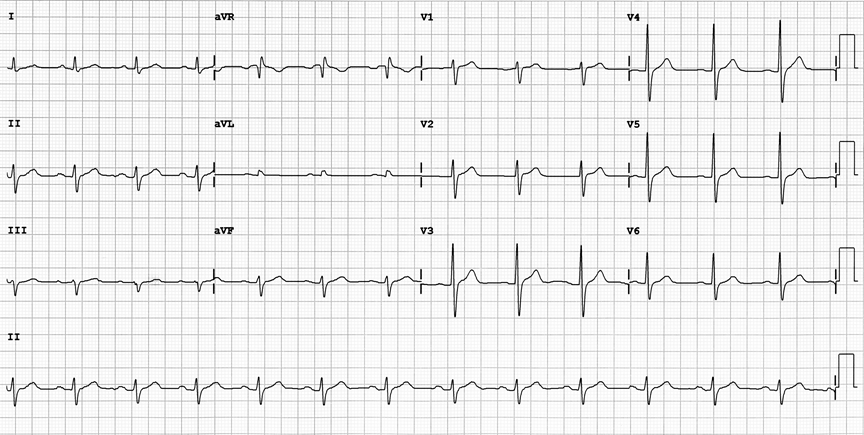
\includegraphics[width=\textwidth]{../assets/ecg-paper-example}
    \bicaption{一张10秒12导联的常规心电图}{A 10-second 12-lead standard ECG}
    \label{fig:ecg-paper-example}
\end{figure}

动态心电图则是在患者进行日常生活活动时记录的心电图。动态心电图的记录可以在几乎任何环境进行,只需要患者佩戴动态心电记录仪(Holter monitor)即可。动态心电记录仪是一种便携式可穿戴设备,可在较长时间内(24小时以上)记录心脏的电活动,有助于检出非持续性心律失常。统计显示,动态心电图在临床诊断中对心肌缺血及各种心律失常事件的检出率都明显高于常规心电图\cite{zhengDongtaixindiantuyuchangguixindiantuzhenduanguanxinbinghuanzhexinjiquexiejixinlushichangdelinchuangxiaoguobijiao2011}。

\subsection{心电自动分析技术}\label{subsec:automatic-analysis}

动态心电图的数据量远远超过常规心电图,在显著提升了诊断精度的同时,也大幅提高了人工诊断的难度。人工进行大量数据的诊断识别,不仅使得医生过于疲劳、容易出错,也难以进行实时监测。于是,心电自动分析技术的需求就显而易见了。

心电自动分析是指在采集到的心电信号的基础上,通过对其处理提取表征心脏状态的波形信息和特征参数,获取心脏工作状态的相关信息,然后利用这些特征信息分析、判别心电信号类型及所对应的疾病类型或健康水平,进而对心脏状态和健康状况进行预测\cite{jiXindianxinhaozidongfenxiguanjianjishuyanjiu2006}。

自动化的心电分析算法可以快速、准确地处理心电信号,为专业医疗人员节省时间,提高医疗服务的效率,降低医疗成本。此外,心电自动分析技术也更方便对患者进行实时监测,通过对心电数据进行实时分析可以及时发现患者的异常状况,为患者提供随时随地的医疗监护,降低心血管疾病对患者健康的威胁。


\section{国内外\app 现状}\label{sec:status}

当前国内外已有不少\app ,其中一些使用了人工编写的传统心电分析算法\cite{zhengJiyukechuandaishebeideyidongjianhuAPP2019,wuYidongxindianjiancexitongdeyanjiuyushixian2018,chenYidongxindianxinxijianhuxitongjixindianjiancesuanfadeyanjiu2018,heJiyuyidongpingtaidexindianjianceyiliaoxitongdeshixian2017,gradlRealtimeECGMonitoring2012,wenRealtimeECGTelemonitoring2008},包括自适应双阈值法\cite{chenYidongxindianxinxijianhuxitongjixindianjiancesuanfadeyanjiu2018}、Pan-Tompkins算法\cite{gradlRealtimeECGMonitoring2012}以及一些原创的或基于已有算法改进的未命名的算法等;另一些\app 则使用了深度学习模型\cite{wangJiyushenduxuexideyidongyuanchengxindianjiancexitongshejiyushixian2020,singhSmartECGMonitoring2022,chenJiyushenduxuexidexindianfenximoxingdeshejiyuyouhua2021,liuJiyuyidongzhongduanfenxidekechuandairouxingxindianjiancexitong2021,wangEnablingSmartPersonalized2014,jinPredictingCardiovascularDisease2009}。

使用了深度学习模型的这些\app 按其整体架构可以大致分为两类:一类是在移动端只对数据进行简单统计处理,完整的算法模型则部署于服务端\cite{wangJiyushenduxuexideyidongyuanchengxindianjiancexitongshejiyushixian2020,singhSmartECGMonitoring2022},患者如果想获取完整的分析报告,则需要将数据上传至服务端后,等待服务端分析完成;这种应用架构的主要缺点是,患者能在移动端立即获取的结果较少,而完整分析结果可能因为网络质量差、服务端算力不足等原因而有较大延迟;另外,虽然患者不需要在自己的设备上运行相关算法,节省了一定开销,但上传与下载数据消耗的电量与流量成本不可忽视。另一类应用则采用了边缘计算架构,将深度学习模型部署在移动端,数据分析直接在移动端进行\cite{chenJiyushenduxuexidexindianfenximoxingdeshejiyuyouhua2021,liuJiyuyidongzhongduanfenxidekechuandairouxingxindianjiancexitong2021,wangEnablingSmartPersonalized2014,jinPredictingCardiovascularDisease2009},这样可以缩短延迟,节省带宽,并节省了高算力服务器的成本;然而,已有的少数此类应用都只实现了极简单的功能,旨在以演示程序验证模型正确性,并没有进行完整的应用开发,如图~\ref{fig:demos} 所示;此外,这些简单的演示程序均只进行了单一操作系统的开发。

\begin{figure}[ht]
    \subcaptionbox{\cite{chenJiyushenduxuexidexindianfenximoxingdeshejiyuyouhua2021}}{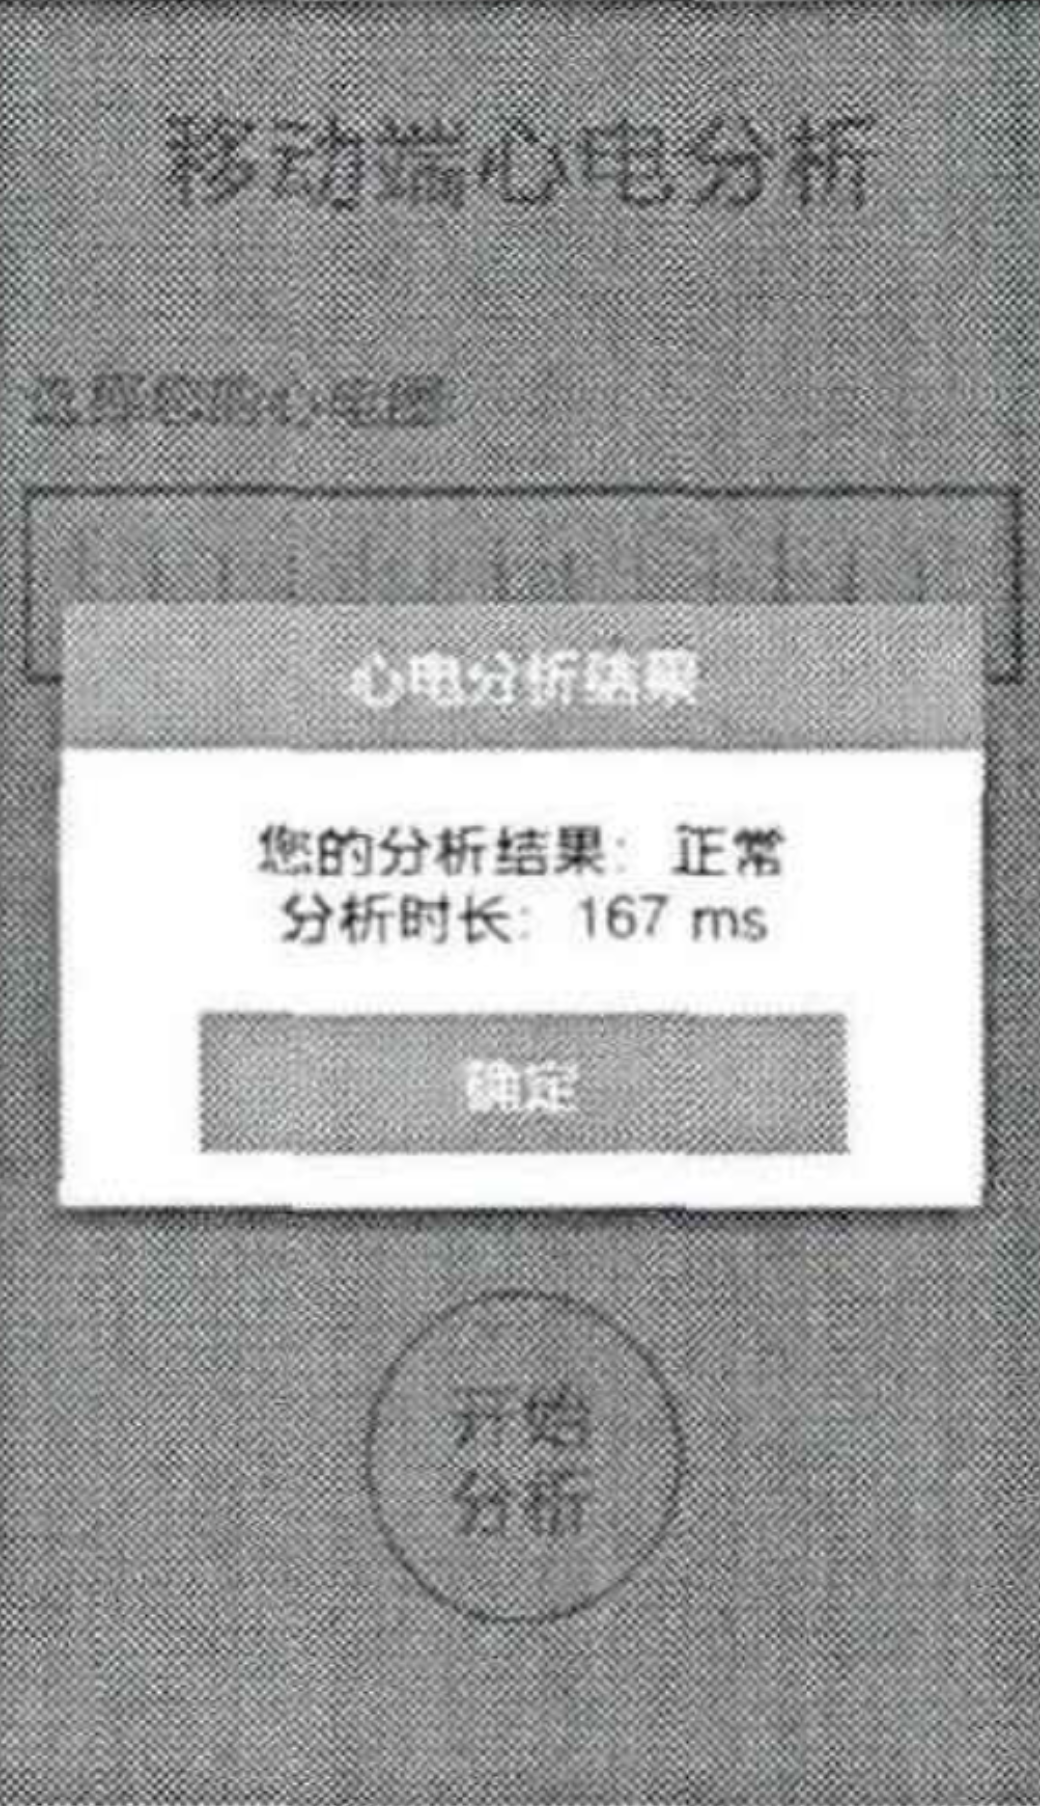
\includegraphics[height=9cm]{../assets/demo-0}}
    \subcaptionbox{\cite{liuJiyuyidongzhongduanfenxidekechuandairouxingxindianjiancexitong2021}}{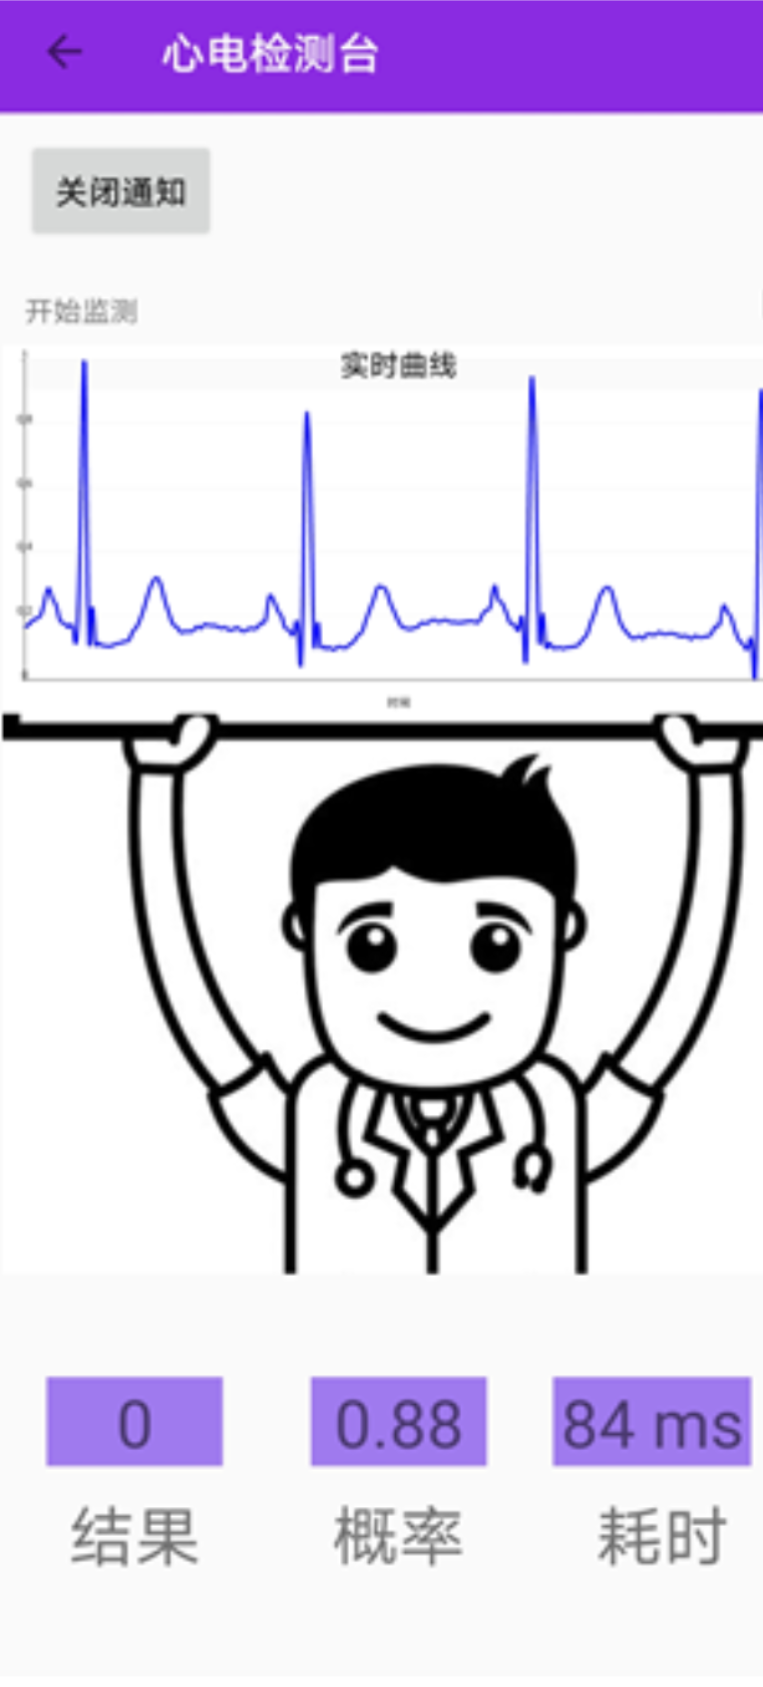
\includegraphics[height=9cm]{../assets/demo-1}}
    \subcaptionbox{\cite{jinPredictingCardiovascularDisease2009}}{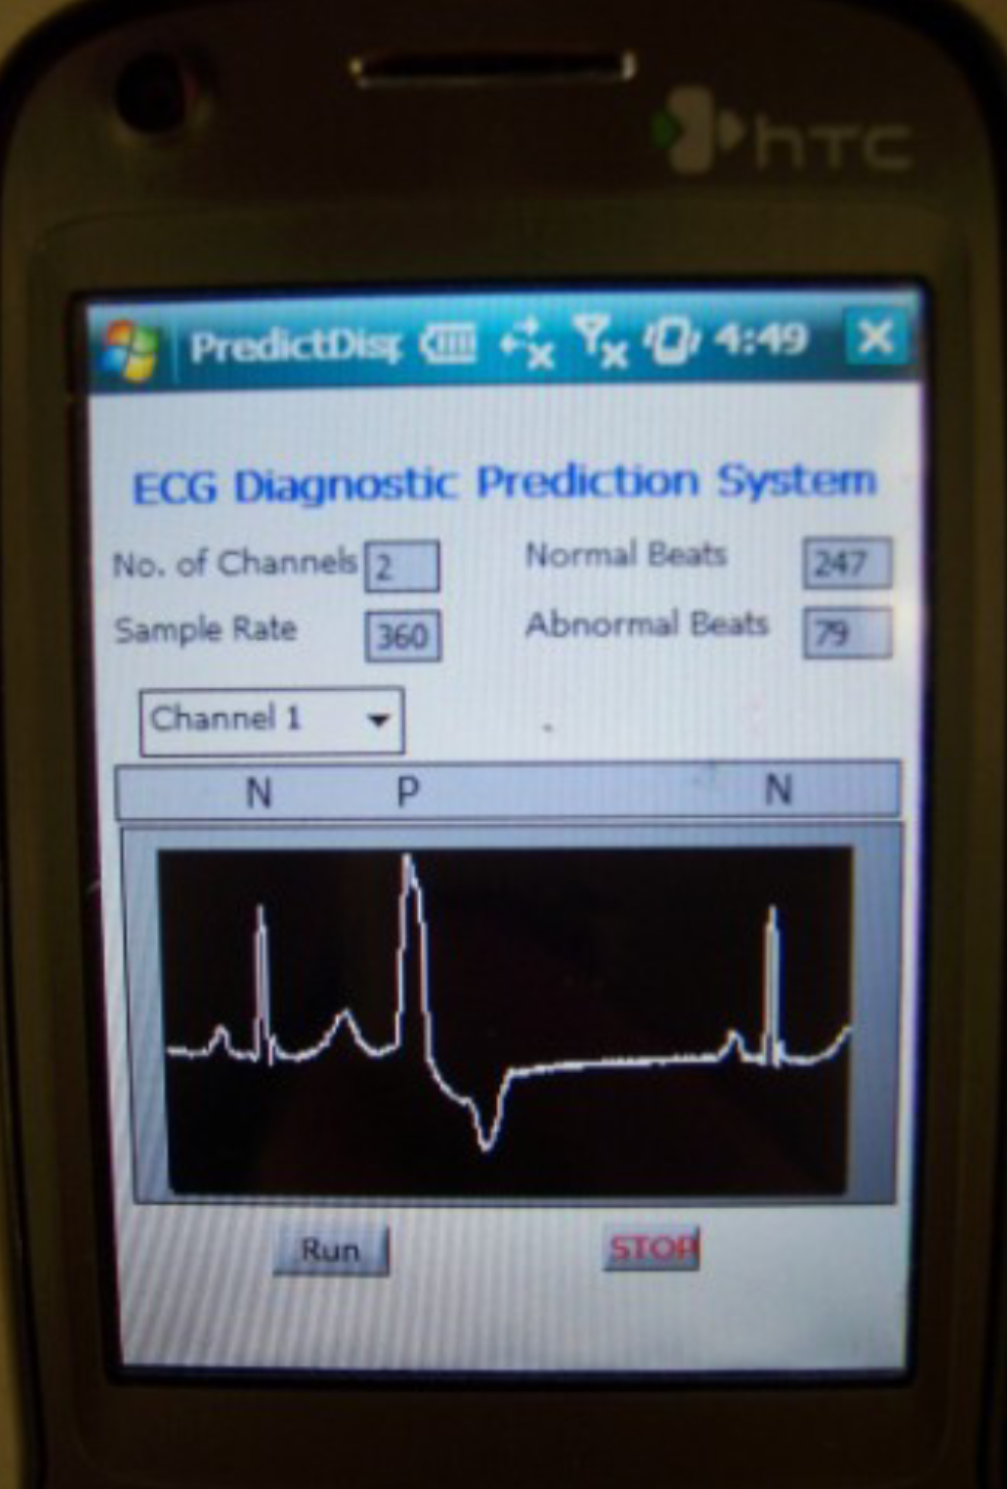
\includegraphics[height=9cm]{../assets/demo-2}}
    \bicaption{一些仅为验证模型而开发的简单演示程序}{Some demo programs only for model validation}
    \label{fig:demos}
\end{figure}


\section{本项目的主要工作}\label{sec:work}

本项目与~\ref{sec:status} 节中所述的最后一类相似,也就是采用边缘计算架构,将深度学习模型部署在移动端,数据分析直接在移动端进行。本项目与上文提及的已有的同类应用的主要差别在于其选题来源于导师的心电图课题的子项目,是在已经基于PyTorch完成了相关算法模型\cite{songDongtaixindiantudezhinengjiancesuanfayanjiuyuyingyong2022}的情况下进行的,在项目之初就已有较好的人工智能算法模型的技术支撑。于是,相比于偏重算法研究而在实际的应用开发方面较为欠缺的其他项目,本项目的主要工作在于将已有的算法模型与移动应用开发技术进行整合,以实现一个较为完整的\app ,目标是最终投入到实际的生产环境中供患者使用。更具体地说,本项目主要做了以下工作:

\todo{后面几章写完具体工作再回来细化下这部分。}


\section{论文组织结构}\label{sec:structure}

\todo{写完各章内容之后再总结下组织结构。}
